\addcontentsline{toc}{chapter}{Implementation}
\chapter*{Implementation}
\addcontentsline{toc}{section}{Code}
\section*{Code in python:}

\addcontentsline{toc}{section}{Screenshot}
\begin{verbatim}
        import time
        import random
        import matplotlib.pyplot as plt
        
        # Define the sorting algorithms
        
        def quicksort(arr):
            if len(arr) <= 1:
                return arr
            pivot = arr[0]
            left = [x for x in arr[1:] if x < pivot]
            right = [x for x in arr[1:] if x >= pivot]
            return quicksort(left) + [pivot] + quicksort(right)
        
        def mergesort(arr):
            if len(arr) <= 1:
                return arr
            mid = len(arr) // 2
            left = mergesort(arr[:mid])
            right = mergesort(arr[mid:])
            result = []
            i, j = 0, 0
            while i < len(left) and j < len(right):
                if left[i] < right[j]:
                    result.append(left[i])
                    i += 1
                else:
                    result.append(right[j])
                    j += 1
            result += left[i:]
            result += right[j:]
            return result
        
        def heapify(arr, n, i):
            largest = i
            left = 2*i + 1
            right = 2*i + 2
            if left < n and arr[left] > arr[largest]:
                largest = left
            if right < n and arr[right] > arr[largest]:
                largest = right
            if largest != i:
                arr[i], arr[largest] = arr[largest], arr[i]
                heapify(arr, n, largest)
        
        def heapsort(arr):
            n = len(arr)
            for i in range(n//2 - 1, -1, -1):
                heapify(arr, n, i)
            for i in range(n-1, 0, -1):
                arr[i], arr[0] = arr[0], arr[i]
                heapify(arr, i, 0)
            return arr
        
        def cocktailsort(arr):
            n = len(arr)
            swapped = True
            start = 0
            end = n-1
            while swapped:
                swapped = False
                for i in range(start, end):
                    if arr[i] > arr[i+1]:
                        arr[i], arr[i+1] = arr[i+1], arr[i]
                        swapped = True
                if not swapped:
                    break
                swapped = False
                end -= 1
                for i in range(end-1, start-1, -1):
                    if arr[i] > arr[i+1]:
                        arr[i], arr[i+1] = arr[i+1], arr[i]
                        swapped = True
                start += 1
            return arr
        
        # Generate random arrays to sort
        
        sizes = [10000, 50000, 100000, 200000, 500000]
        arrays = {}
        for size in sizes:
            arrays[size] = [random.randint(1, size) for _ in range(size)]
        
        # Sort the arrays with each algorithm and record the runtimes
        
        quicksort_times = []
        mergesort_times = []
        heapsort_times = []
        cocktailsort_times = []
        
        for size in sizes:
            array = arrays[size]
            start_time = time.time()
            quicksort(array)
            end_time = time.time()
            quicksort_times.append(end_time - start_time)
        
            array = arrays[size]
            start_time = time.time()
            mergesort(array)
            end_time = time.time()
            mergesort_times.append(end_time - start_time)
        
            array = arrays[size]
            start_time = time.time()
            heapsort(array)
            end_time = time.time()
            heapsort_times.append(end_time - start_time)
        
            array = arrays[size]
            start_time = time.time()
            cocktailsort(array)
            end_time = time.time()
            cocktailsort_times.append(end_time - start_time)
        
        
        plt.plot(sizes, quicksort_times, label="Quicksort")
        plt.plot(sizes, mergesort_times, label="Mergesort")
        plt.plot(sizes, heapsort_times, label="Heapsort")
        plt.plot(sizes, cocktailsort_times, label="Cocktailsort")
        plt.xlabel("Array Size")
        plt.ylabel("Runtime (Seconds)")
        plt.legend()
        plt.show()
        
\end{verbatim}
\section*{Screenshot:}
{ \centering 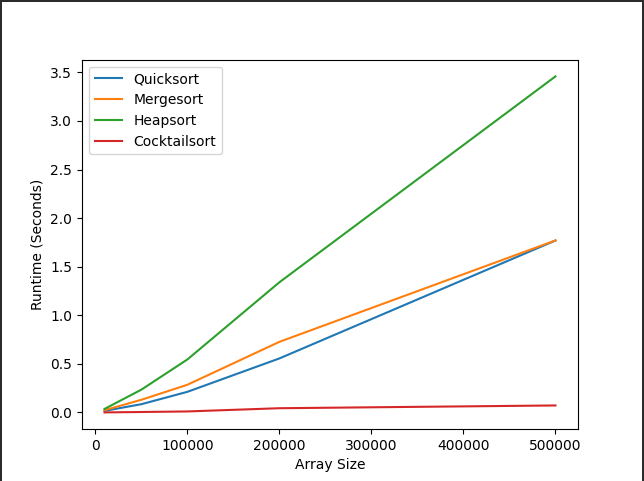
\includegraphics[width=\textwidth]{images/lab.png} }